\chapter{Research Proposal}\label{chap:research_proposal}

This chapter will provide an overview of the problem this thesis is trying to solve. First, the existing methods for initial flow estimation will be presented in Sections \ref{sec:multivp} and \ref{sec:ml_initial_flow}. Next, in Section \ref{sec:prelim_data_analysis}, a preliminary analysis of the input data used in both approaches is undertaken. With the problems identified in the previous section, a hypothesis and research questions are proposed in Section \ref{sec:hypothesis}, intending to solve these issues. Finally, the methodology and development plans are proposed in Sections \ref{sec:method} and \ref{sec:work_plan}, respectively.

\section{MULTI-VP}\label{sec:multivp}

MULTI-VP \cite{pinto.rouillard_MultipleFluxtubeSolar_2017} is a global MHD model that simulates the three-dimensional structures of the solar wind. In addition, it also estimates the conditions at the Sun's chromosphere, transition region, corona, and low heliosphere. The model computes many one-dimension solar wind solutions from full flux-tube geometries and heating functions. Background magnetic field geometries are extrapolated from publicly available magnetogram data. The method can estimate solar wind profiles across the Sun's entire atmosphere up to 30 solar radii. The results directly link the geometry of magnetic flux tubes in the lower corona with the distributions of fast and slow solar wind flows. MULI-VP proved faster than other MHD models and did not suffer from cross-field diffusion effects.

The magnetogram data used as input to the MULTI-VP model comprises the six columns in Table \ref{tab:multivp_columns}, each with 640 rows ordered by distance to the Sun. The first three columns serve as the input to the model where $R$ is the radial coordinate radius, $B$ is the magnetic field, and $\alpha$ indicates the inclination of the flux tube. In addition, the simulator also takes the initial expert estimates (last three columns) as input, approximating better solutions during the simulation. $n$ indicates the number of protons per unit volume, $v$, the speed-oriented along the line, and $T$, the temperature at that point in space. 


\begin{table}[ht]
    \caption{Data columns of magnetogram used by MULTI-VP.}
    \label{tab:multivp_columns}
    \begin{subtable}[h]{0.32\textwidth}
        \centering
        \begin{tabular}{lcc}
        \hline
        \multicolumn{3}{c}{Input (Partial Flows)}                              \\ \hline
        $R${[}$R_{sun}${]} & $B${[}$G${]} & $\alpha${[}$deg${]} \\ \hline
        \end{tabular}
    \end{subtable}
    \begin{subtable}[h]{0.32\textwidth}
        \centering
        \begin{tabular}{ccc}
        \hline
        \multicolumn{3}{c}{Output (Estimations)}                           \\ \hline
        $n${[}$cm^{-3}${]} & $v${[}$km/s${]} & $T${[}$MK${]} \\ \hline
        \end{tabular}
    \end{subtable}
\end{table}

A representation of the data processing of MULTI-VP can be seen in Figure \ref{fig:multivp_method}. As previously stated, MULTI-VP takes as input partial flow definitions of the solar wind along with initial expert estimations and derives better solutions during simulation.

\vspace{0.5cm}
\begin{figure}[!h]
\centering
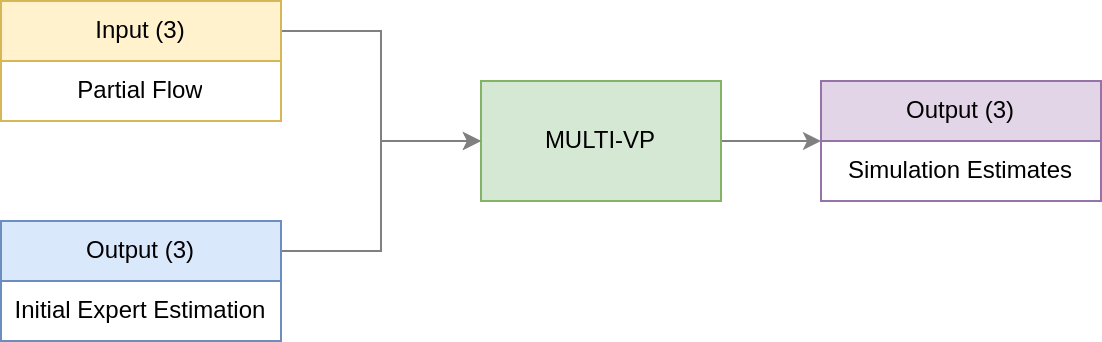
\includegraphics[width=0.8\textwidth]{figures/multivp_method.png}
\caption[MULTI-VP methodology dataflow]{MULTI-VP methodology dataflow. The model takes as input both the partial flow and its associated expert initial guess and then derives a better solution.\label{fig:multivp_method}}
\end{figure}


\section{ML for Initial Flow Estimation}\label{sec:ml_initial_flow}
Due to the complexity and a large number of calculations, MULTI-VP, like other MHD simulations, still takes a long time to reach solar wind solutions. Furthermore, the need for initial expert guesses also significantly delays the process. These factors directly affect the prediction capability and preparation for extreme solar events. Recently in \cite{barros_InitialConditionEstimation_}, it has been proved that machine learning techniques can accurately produce good initial flow estimations that MULTI-VP can later use. The authors also proved that the quality of the flow estimations is directly linked to the total execution time of the simulation. These allow for faster convergence of the MHD simulation as the initial estimates are closer to the final solution. 

The approach, illustrated in Fig. \ref{fig:multivp_rnn}, consists of training an ML model to learn to predict the initial expert estimates from the initial partial flow input. Analogous to the method presented in Section \ref{sec:multivp}, MULTI-VP takes as input the partial flows along with their initial conditions predicted by the ML model.

\begin{figure}[ht]
\centering
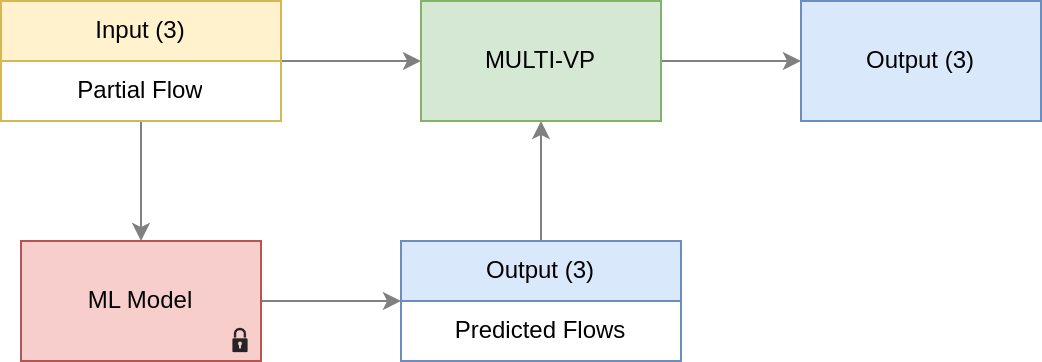
\includegraphics[width=0.8\textwidth]{figures/multivp_rnn.png}
\caption[ML methodology dataflow]{ML methodology dataflow. An ML model estimates the initial conditions of a given partial flow. These are then passed to MULTI-VP, approximating them into a final solution. \label{fig:multivp_rnn}}
\end{figure}

However, the reduction in execution time was minimal as the model, like many other ANN solutions, was very susceptible to noise in the samples used during training. In \cite{barros_InitialConditionEstimation_}, the authors posit that the presence of outliers during the training phase hampered the overall prediction quality of the model.



\section{Anomaly in the Input Data}\label{sec:prelim_data_analysis}
Some preliminary analysis of the input data for the model was carried out to demonstrate the existence of outliers in the data used to train the prediction model of the previous section. The radial profiles of the magnetic field in the function of the radial coordinate radius, $R$, can be seen in Fig. \ref{fig:magnetic_radius_outliers}. It is possible to observe some extreme variations in the data, which indicate the existence of outliers. Additionally, the distribution of magnetic field, $B$ and flux tube inclination values, $\alpha$, are expressed in Figure \ref{fig:input_distrib_bp}. There exist a large number of out-of-distribution samples in the dataset used for training the prediction model.


\begin{figure}[ht]
\centering
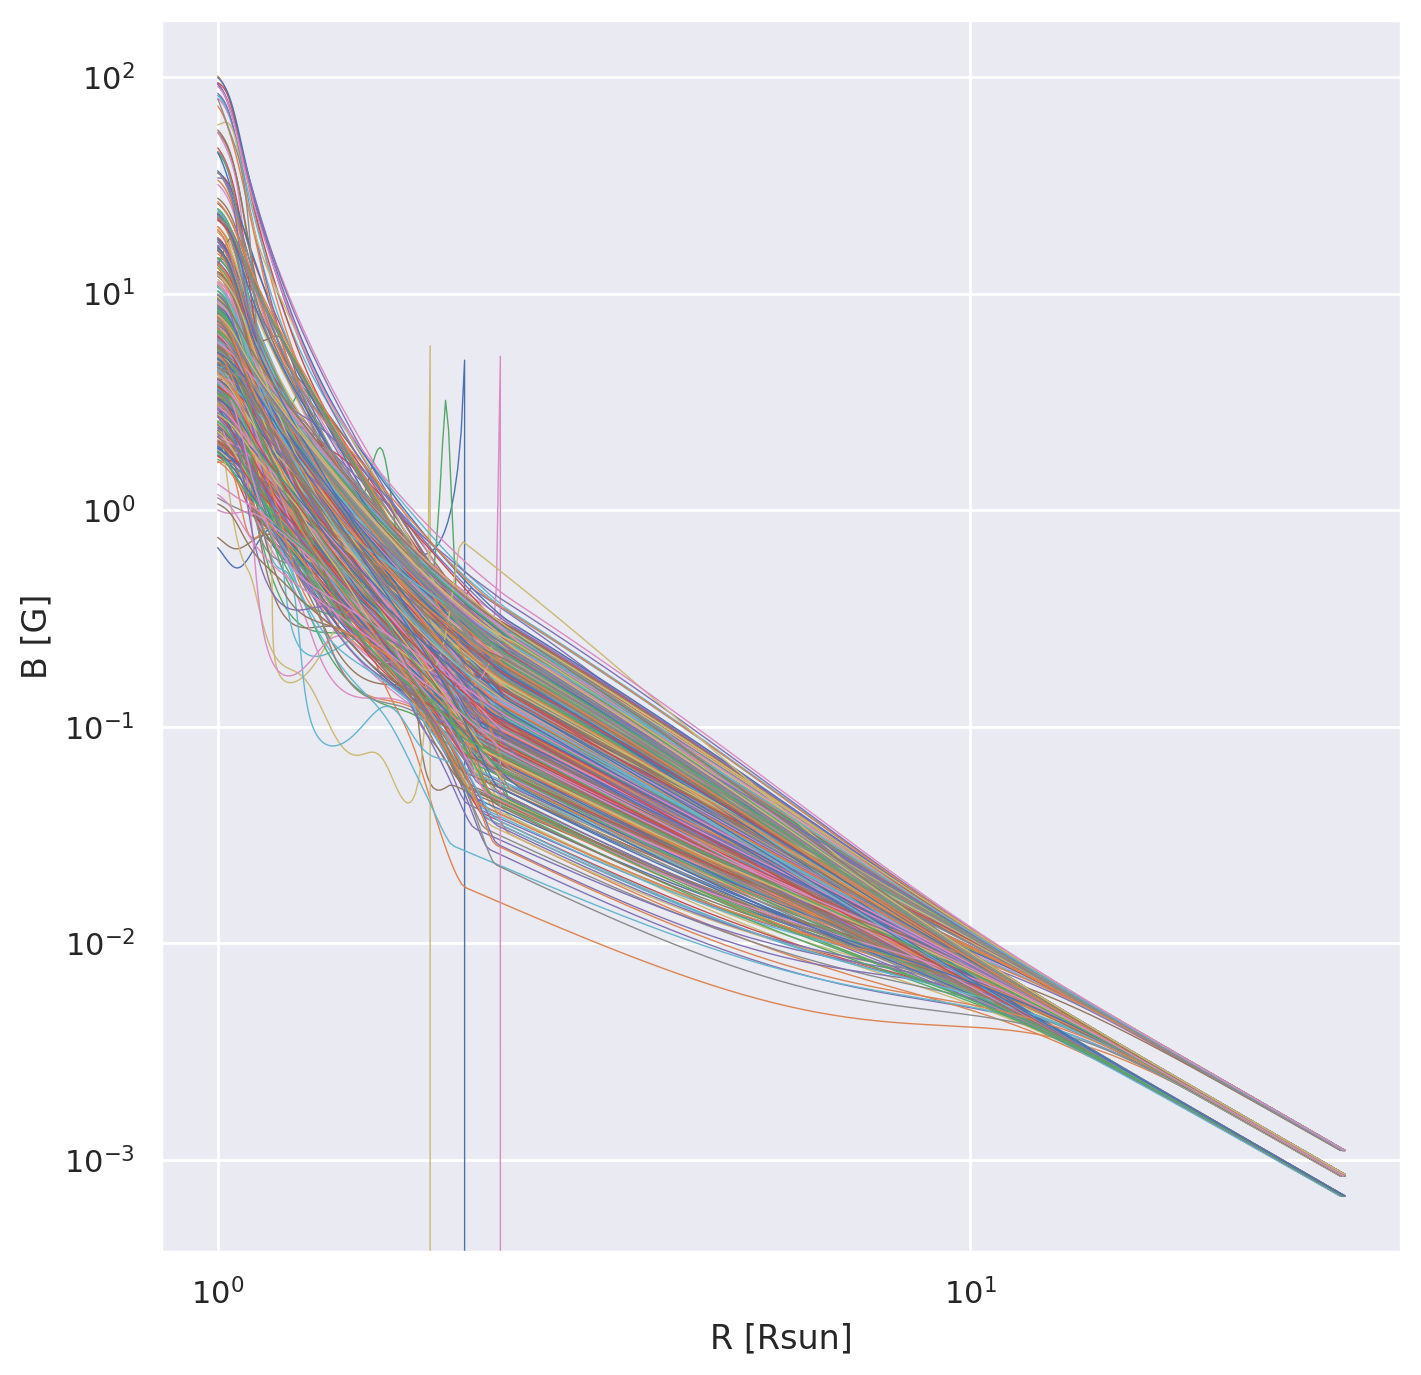
\includegraphics[width=0.5\textwidth]{figures/magnetic_radius_outliers.png}
\caption{Radial profiles of the magnetic field amplitude for the dataset flux-tubes.}
\label{fig:magnetic_radius_outliers}
\end{figure}

\begin{figure}[ht]
     \centering
     \begin{subfigure}[b]{0.32\textwidth}
         \centering
         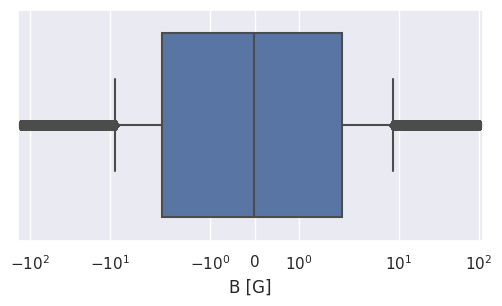
\includegraphics[width=\textwidth]{figures/magnetic_field_boxplot.png}
     \end{subfigure}
     \hfill
     \begin{subfigure}[b]{0.32\textwidth}
         \centering
         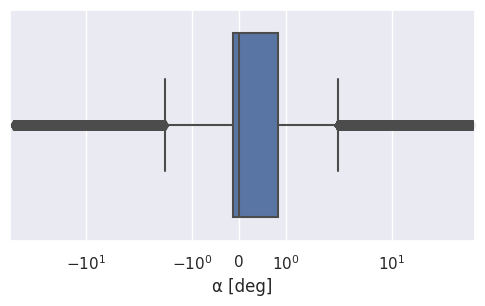
\includegraphics[width=\textwidth]{figures/inclination_bp.png}
     \end{subfigure}
     \hfill
        \caption{Distribution of input values}
        \label{fig:input_distrib_bp}
\end{figure}

A similar process was carried out on the output data (refer to Table \ref{tab:multivp_columns}) to assert if it contained abnormal values that would also affect the training of the ML solution. Significant fluctuations can be observed in all instances of the output columns in Figure \ref{fig:output_distr_plot}. The distribution for the output values can also be seen in Figure \ref{fig:output_distrib_bp}.

\begin{figure}[ht]
     \centering
     \begin{subfigure}[b]{0.32\textwidth}
         \centering
         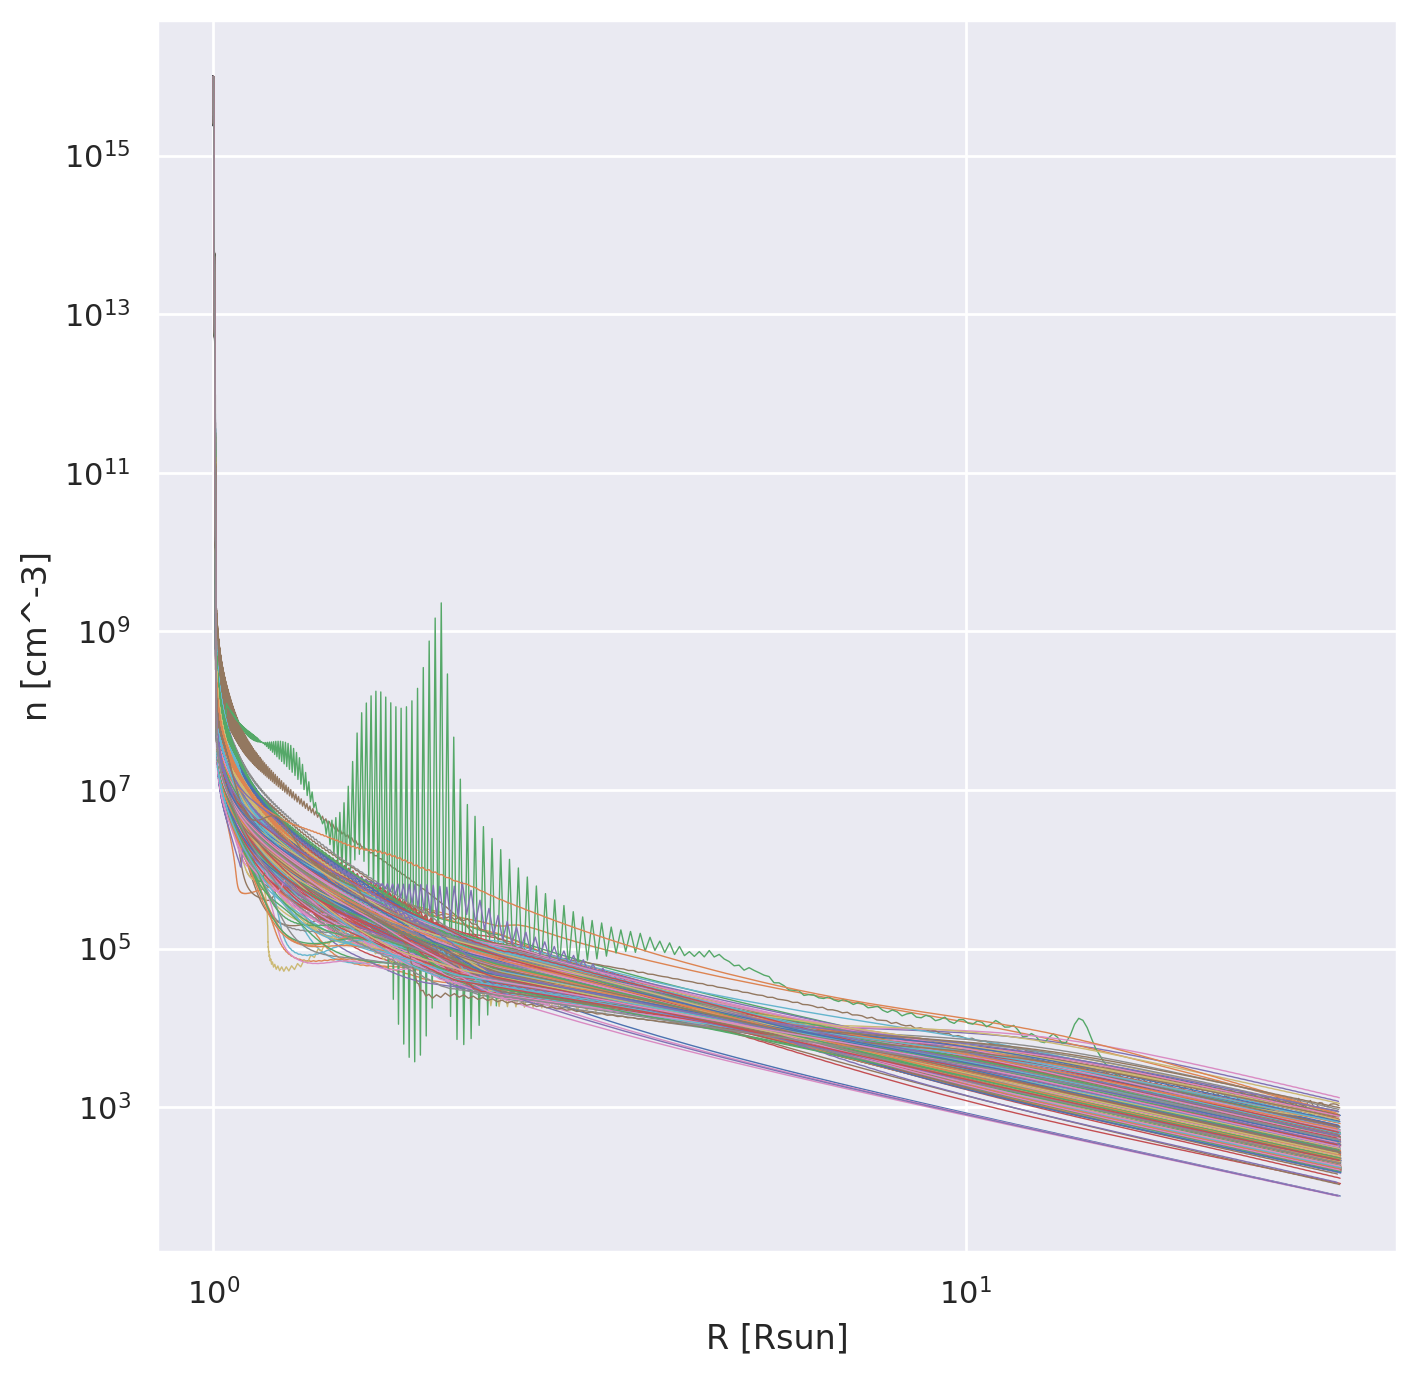
\includegraphics[width=\textwidth]{figures/volume_radius.png}
     \end{subfigure}
     \hfill
     \begin{subfigure}[b]{0.32\textwidth}
         \centering
         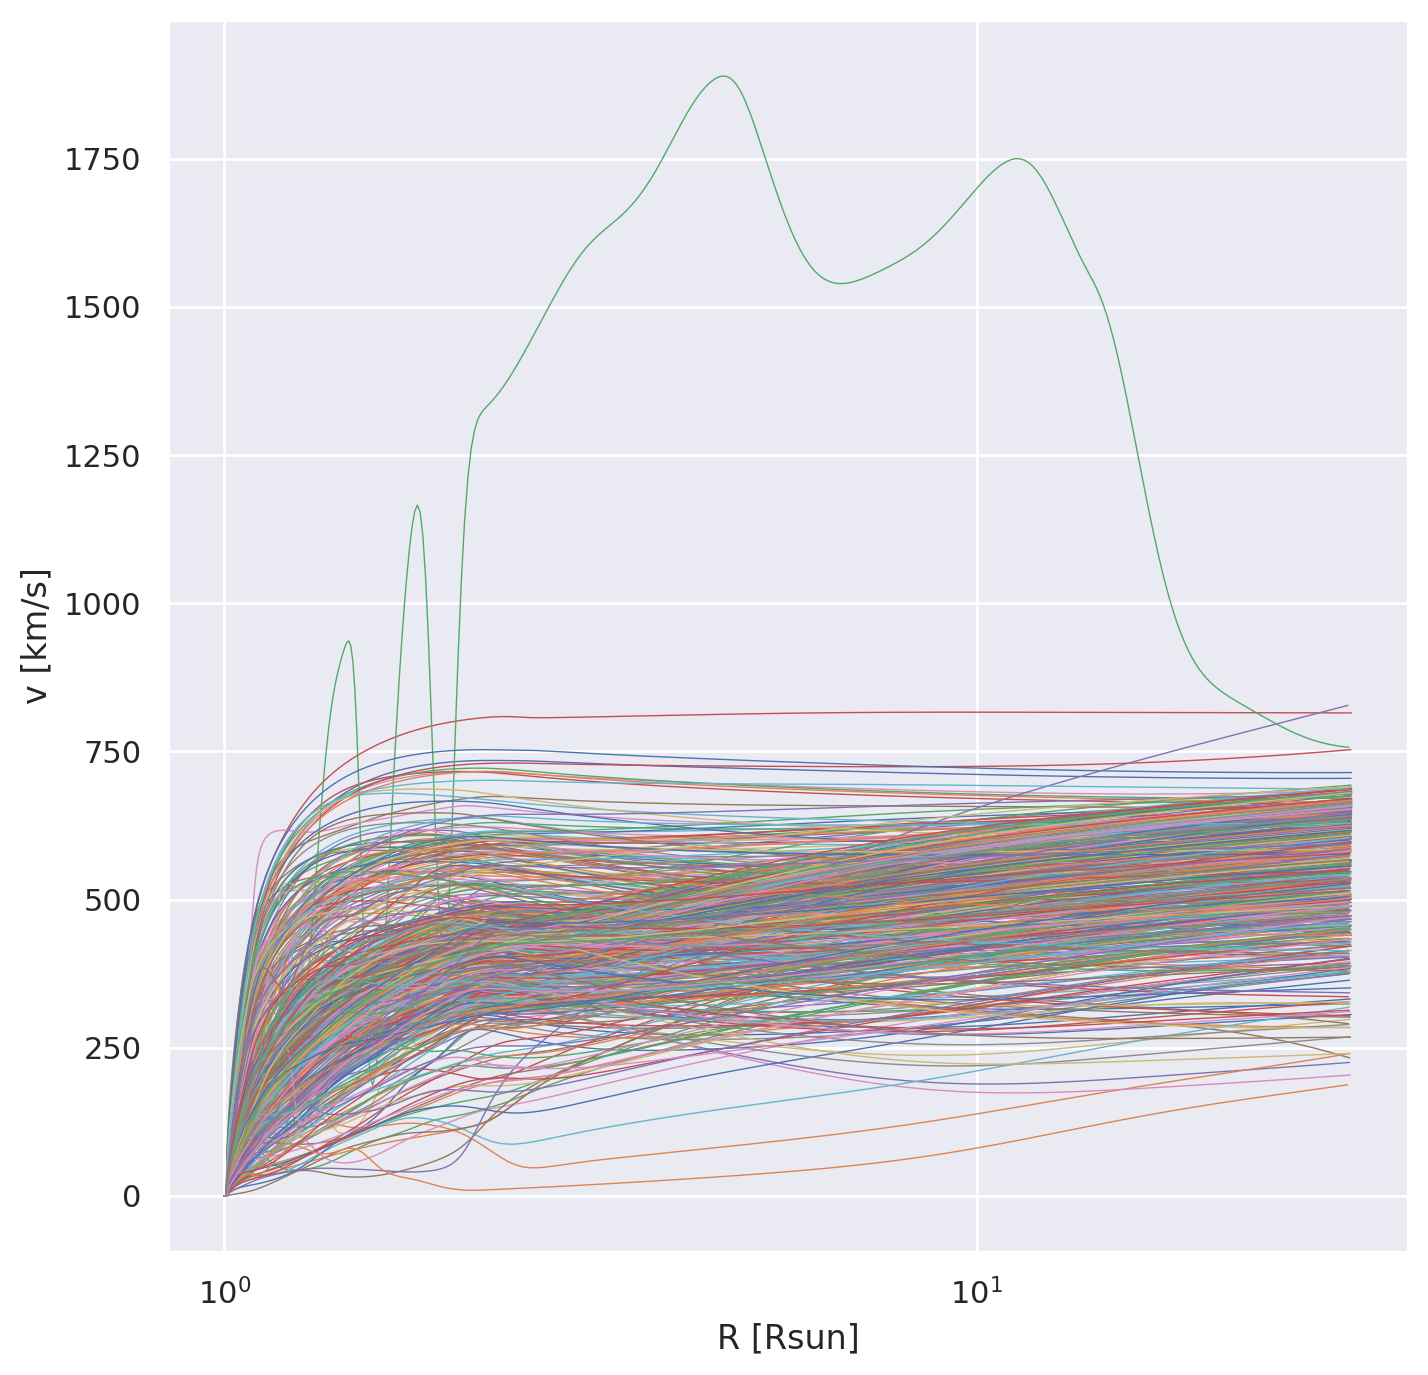
\includegraphics[width=\textwidth]{figures/velocity_radius.png}
     \end{subfigure}
     \hfill
    \begin{subfigure}[b]{0.32\textwidth}
         \centering
         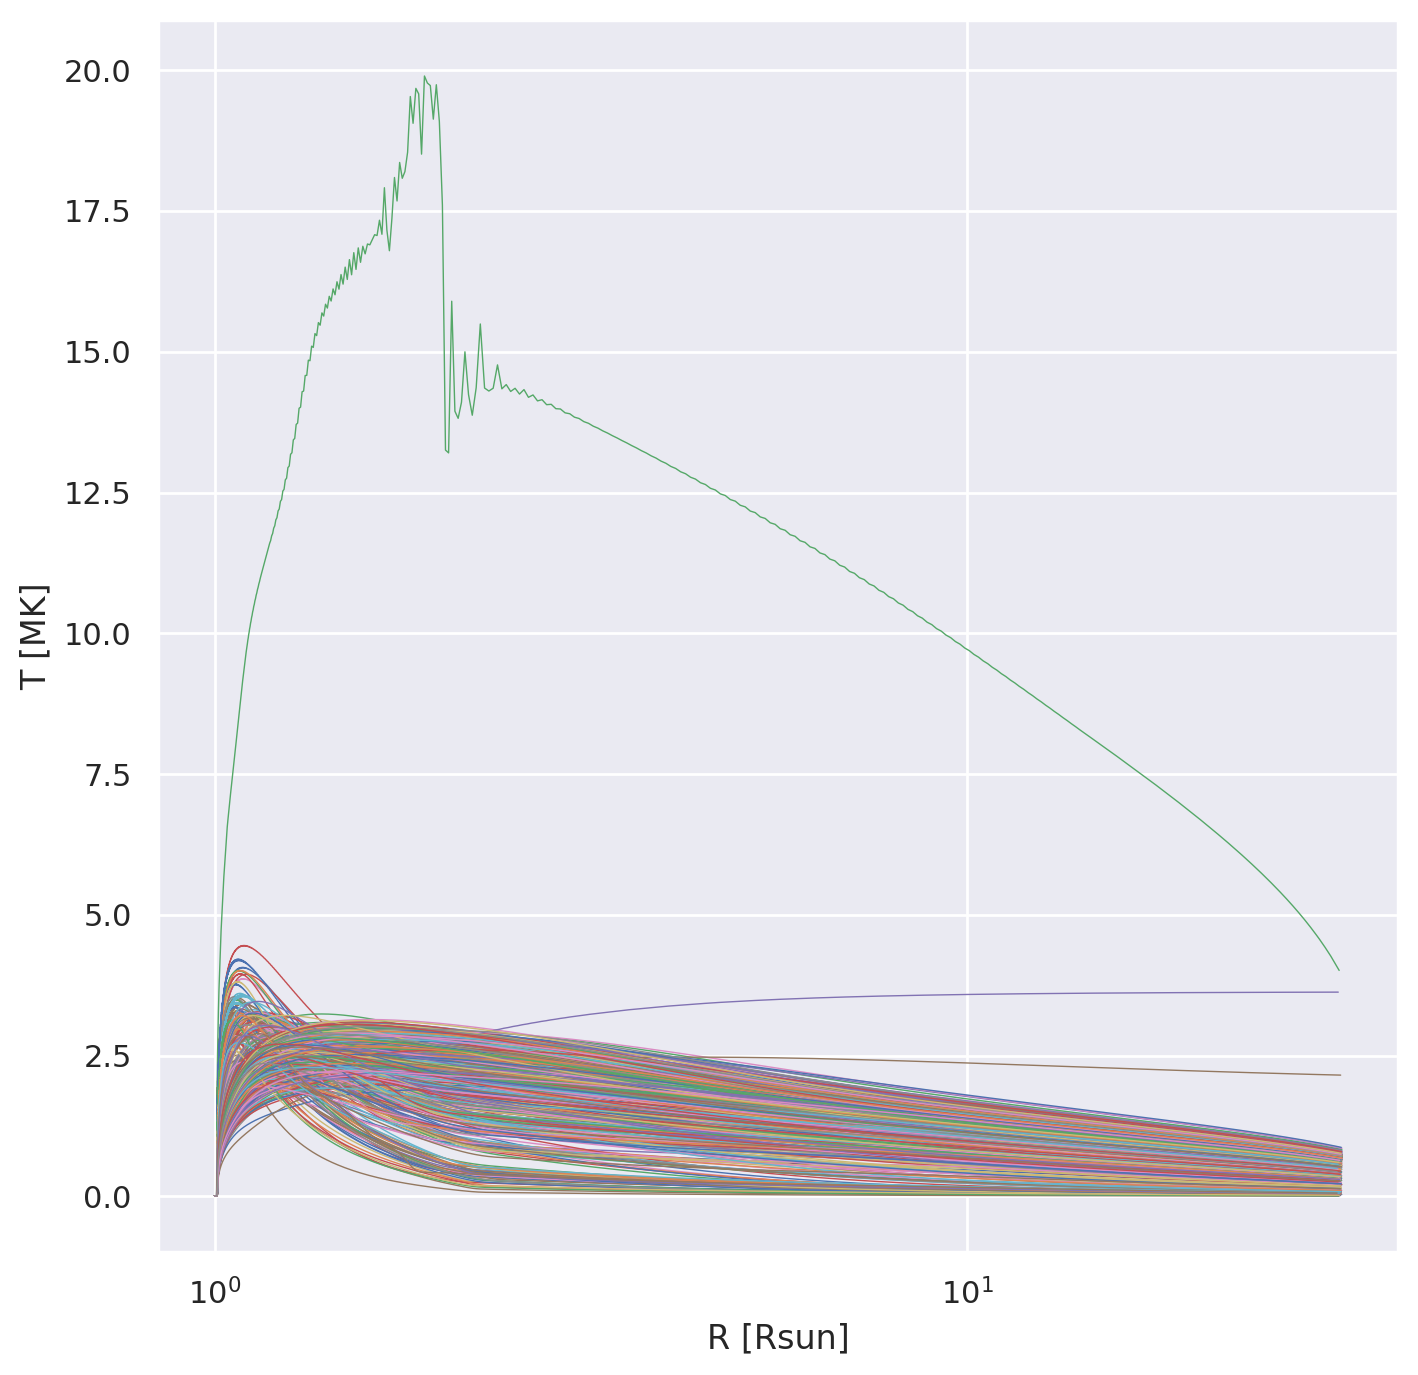
\includegraphics[width=\textwidth]{figures/temperature_radius.png}
     \end{subfigure}
     \hfill
    \caption{Plots of output variables in relation to $R$.}
    \label{fig:output_distr_plot}
\end{figure}

\begin{figure}[ht]
     \centering
     \begin{subfigure}[b]{0.32\textwidth}
         \centering
         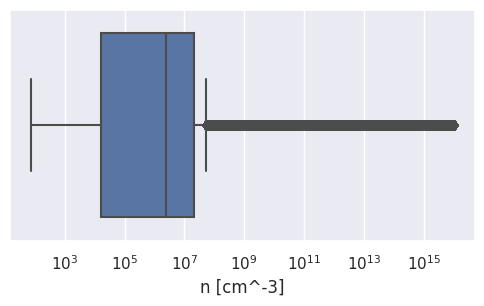
\includegraphics[width=\textwidth]{figures/volume_bp.png}
     \end{subfigure}
     \hfill
     \begin{subfigure}[b]{0.32\textwidth}
         \centering
         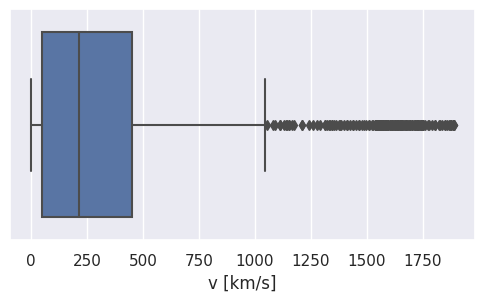
\includegraphics[width=\textwidth]{figures/velocity_bp.png}
     \end{subfigure}
     \hfill
     \begin{subfigure}[b]{0.32\textwidth}
         \centering
         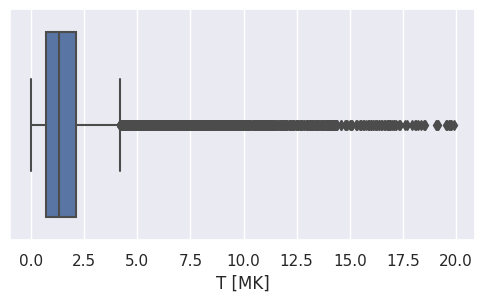
\includegraphics[width=\textwidth]{figures/temperature_bp.png}
     \end{subfigure}
     \hfill
        \caption{Distribution of outputs used during the training of the predictive model.}
        \label{fig:output_distrib_bp}
\end{figure}


\section{Hypothesis}\label{sec:hypothesis}
Taking these problems into consideration, this thesis aims to evaluate the following hypothesis:
\begin{adjustwidth}{2cm}{}
    GAN-based anomaly detection architectures can accurately and automatically detect outliers in the solar wind profiles data used to train the NN model for initial condition estimation and improve the model's predictions.
\end{adjustwidth}

We will try to validate this hypothesis by (1) verifying that the dataset after outlier removal significantly improves the prediction quality of the RNN and (2) if the predictions with a normalized dataset reduce the time that MULTI-VP takes to reach a solution.

To validate the proposed hypothesis, the following research questions were defined:

\begin{description}
    \item[RQ1] \textit{Can GAN-based architectures accurately detect outliers in solar wind profiles?} Considering outlier samples as the positive class, we are mostly trying to reduce the False Negative Rate (FN), which causes the worst effects in the predictive model training. As a secondary priority, we will focus on reducing the amount of False Positives (FP) to ensure that almost no relevant samples are excluded from the training process.
    \item[RQ2] \textit{Does the resulting dataset significantly improve the predictive ability of the RNN?} If the resulting dataset after the removal of outliers results in an improvement in the model used to predict initial conditions from input flows. In other words, the mean square distance between the real estimations and the ones predicted by the model is less than with the previous method.
    \item[RQ3] \textit{Does the improved predictive ability of the RNN result in a further reduction of execution time for MULTI-VP?} This question aims to clarify if the developed model for initial flow estimation can produce better approximations of solar wind flows and thus reduce the time it takes for MULTI-VP to reach a solution.
\end{description}

\section{Methodology}\label{sec:method}
To evaluate the veracity of the hypothesis, we propose developing a GAN architecture to detect outliers in magnetogram files with an approach similar to the ones in \cite{li.etal_MADGANMultivariateAnomaly_2019}, and \cite{bashar.nayak_TAnoGANTimeSeries_2020}. It will use the generator and the discriminator to detect anomalies in the original dataset. 

The GAN will have a similar architecture to the one in \cite{goodfellow.etal_GenerativeAdversarialNets_}. During training, the generator's goal is to synthesize magnetogram samples close to the original distribution of the dataset. The discriminator will be tasked with distinguishing fake magnetograms from real ones. Only inlier samples will be used in this process.

For the detection phase, we propose the methodology in Figure \ref{fig:proposed_gan_arch} with the components trained in the previous phase. First, a sample will be extracted from the dataset and passed directly to the discriminator. If the sample is abnormal, it will probably have a higher loss than normal ones, as the discriminator is only trained on the normal data distribution. Next, the sample is mapped into the latent space, where one of the methods from \cite{li.etal_MADGANMultivariateAnomaly_2019} or \cite{bashar.nayak_TAnoGANTimeSeries_2020} could be used. The resulting latent sample is then fed to the generator, which is tasked with reconstructing it. In the next step, the reconstructed sample is compared with the real one, and the reconstruction error is calculated. In theory, if the real sample is an outlier, then the reconstruction error will be much higher when compared to inlier examples, as the generator only learned to generate samples from the normal distribution. In the end, discriminator loss and the reconstruction error will be combined to calculate the anomaly score. The example is considered an anomaly if this score exceeds a predefined threshold.

\begin{figure}[ht]
\centering
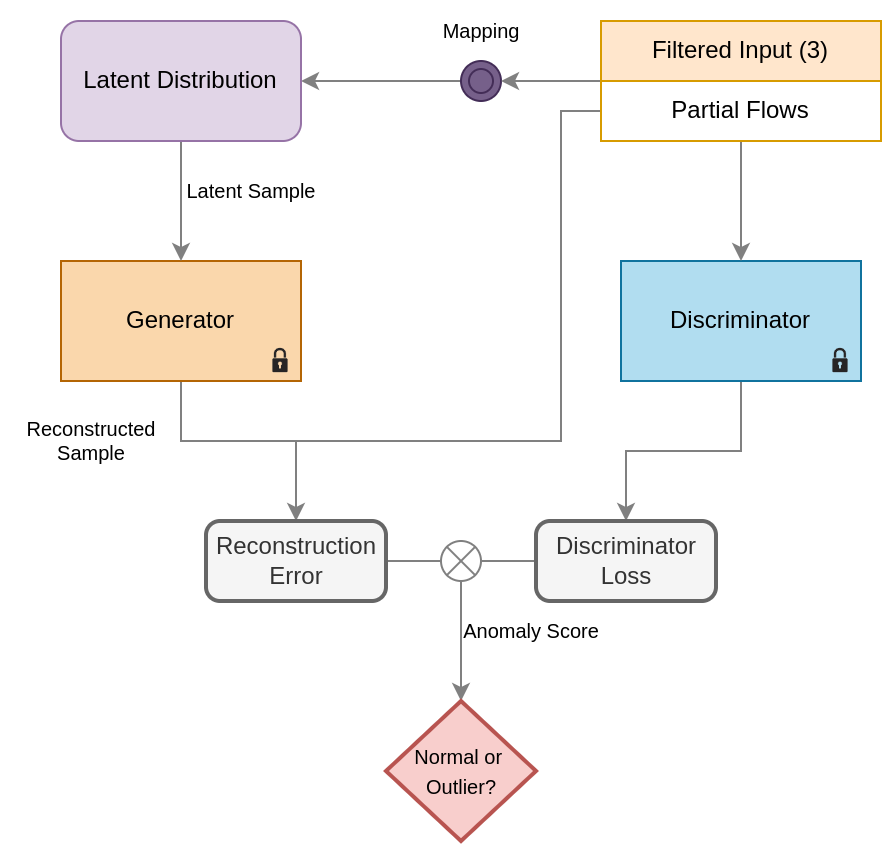
\includegraphics[width=0.8\textwidth]{figures/proposed_gan_arch.png}
\caption{Proposed method for anomaly detection in magnetogram data.}
\label{fig:proposed_gan_arch}
\end{figure}

The developed GAN will be incorporated into the existing ML methodology expressed in Figure \ref{fig:multivp_rnn}. The resulting representation of the overall data flow for the proposed approach can be seen in Figure \ref{fig:gan_rnn_multivp}. The goal is to use a GAN-based solution to detect outlier samples before training the ML models for initial flow estimation. We propose using either the input values of the available magnetograms or a combination of input and outputs (refer to Table \ref{tab:multivp_columns}) for this step.

\begin{figure}[ht]
\centering
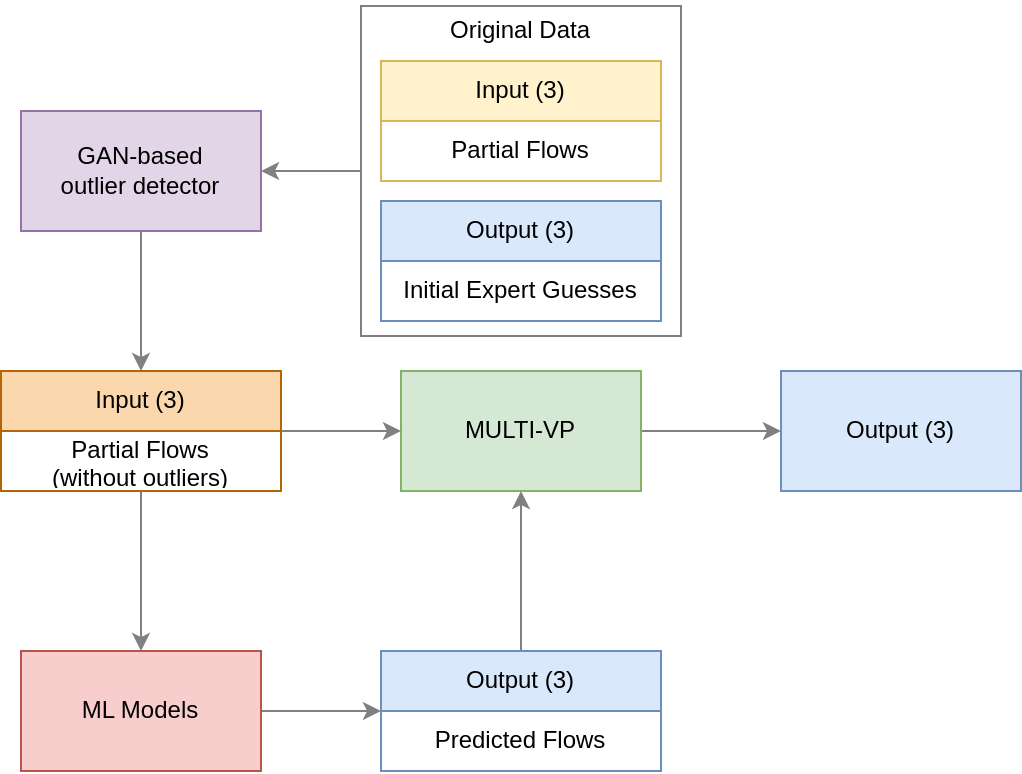
\includegraphics[width=0.8\textwidth]{figures/gan_rnn_multivp.png}
\caption{GAN-based outlier detection method dataflow.}
\label{fig:gan_rnn_multivp}
\end{figure}

The results will be evaluated in an initial step by comparing the distance between the predicted initial estimation of the ML model and the real ones. Similar to the work carried out in \cite{barros_InitialConditionEstimation_}, we will measure the Mean Squared Error (MSE) between the two. Subsequently, the filtered inputs from the outlier detection step will be fed to MULTI-VP along with the initial flow estimations from the ML model. Then the simulation execution times when using the proposed methodology will be compared with the previous implementations to assert if there was a significant reduction.

\section{Work Plan}\label{sec:work_plan}
In Figure \ref{fig:work_plan}, an illustration of the proposed work plan is given. In the initial part of development, several clustering methods will be applied to the dataset to verify if any cluster composition significantly improves the ML model's performance. These methods will be evaluated on the existing model, and then the MSE scores will be compared with the ones obtained with the previous method.

In the next stage, a GAN architecture will be designed to detect outliers in magnetogram data. Pytorch \cite{NEURIPS2019_9015} will be the tool used for this goal. Some time was also allocated to implementing GANs with this framework. After developing a suitable method for outlier detection on the given dataset, an extensive analysis of the performance of the ML model with the data without outliers will be done. This part validates the hypothesis defined in Section \ref{sec:hypothesis}. During this time, some adjustments might have to be made to the initial solution to overcome any shortcomings on these tests. As was already stated, we will use the MSE between the actual estimations and those predicted with the new method. 

After finetuning, the newly improved estimations from the previous step will be used on MULTI-VP to evaluate if the chosen implementation resulted in a shorter execution time. The final stage will be dedicated to writing the dissertation and accommodating any delays from the previous steps.

\begin{figure}[ht]
\centering
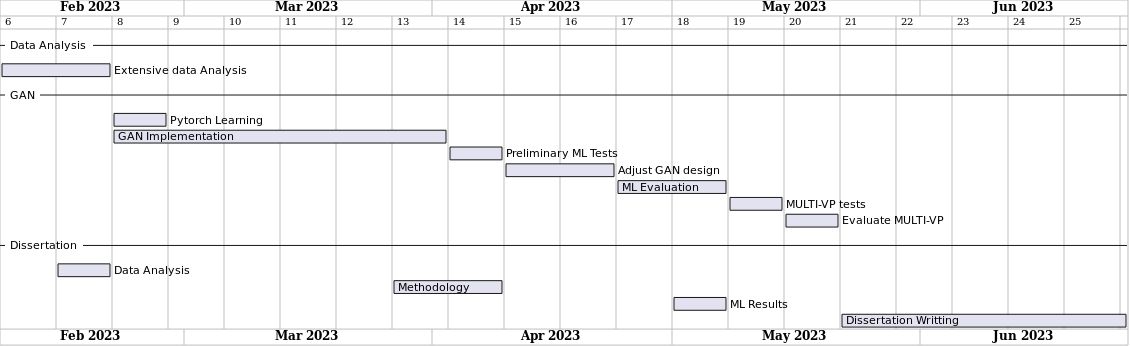
\includegraphics[width=\textwidth]{figures/work_plan.png}
\caption{Proposed development plan.}
\label{fig:work_plan}
\end{figure}
